\documentclass[12pt]{article}

\newcommand{\CiteMathPackage}{../../math}
\newcommand{\CiteReference}{../reference.bib}

% Packages
\usepackage{setspace,amsmath,amsfonts,amssymb,amsthm,fancyvrb,soul}
\usepackage{epstopdf,marginnote,datetime,enumitem,rotating}
\usepackage{graphicx,threeparttable,booktabs,float}

% Page Setup
\usdate
\usepackage{geometry}
\geometry{scale=0.8}
\usepackage{titlesec}
\titleformat{\paragraph}[runin]{\itshape}{}{}{}[.]
\titlelabel{\thetitle.\;}
\usepackage{indentfirst}
\setlength{\parindent}{10pt}
\setlength{\parskip}{10pt}
\AtBeginDocument{\addtocontents{toc}{\protect\setlength{\parskip}{5pt}}}
\usepackage{Alegreya}
\usepackage[T1]{fontenc} 		 

%% Bibliography
\usepackage{natbib,fancybox,url,xcolor}
\definecolor{MyBlue}{rgb}{0,0.2,0.6}
\definecolor{MyRed}{rgb}{0.4,0,0.1}
\definecolor{MyGreen}{rgb}{0,0.4,0}
\definecolor{MyPink}{HTML}{E50379}
\newcommand{\highlightR}[1]{{\emph{\color{MyRed}{#1}}}} 
\newcommand{\highlightB}[1]{{\emph{\color{MyBlue}{#1}}}}
\newcommand{\highlightP}[1]{{\emph{\color{MyPink}{#1}}}}
\usepackage[bookmarks=true,bookmarksnumbered=true,colorlinks=true,linkcolor=MyBlue,citecolor=MyRed,filecolor=MyBlue,urlcolor=MyGreen]{hyperref}
\bibliographystyle{econ}

%% Theorem Environment
\theoremstyle{definition}
\newtheorem{assumption}{Assumption}
\newtheorem{definition}{Definition}
\newtheorem{theorem}{Theorem}
\newtheorem{proposition}{Proposition}
\newtheorem{lemma}[theorem]{Lemma}
\newtheorem{example}[theorem]{Example}
\newtheorem{corollary}[theorem]{Corollary}
\usepackage{mathtools}
\usepackage{\CiteMathPackage}

\begin{document}

%??%??%??%??%??%??%??%??%??%??%??%??%??%??%??%??%??%??%??%??%??%??%??%??%??%??
%?? Title
%??%??%??%??%??%??%??%??%??%??%??%??%??%??%??%??%??%??%??%??%??%??%??%??%??%??

\title{\bf Comparative Advantage, Learning, and Sectoral Wage Determination, Journal of Labor Economics, 2005}
\author{Wenzhi Wang \thanks{This note is written in my MPhil period at the University of Oxford.} } 
\date{\today}
\maketitle

\citet{gibbonsComparativeAdvantageLearning2005}

\section{Introduction}

We analyze the theoretical and econometric implications of comparative advantage and learning for the wages and sector affiliations of individuals and for changes in these variables over workers' careers. After developing the theory and econometrics, we turn to two empirical applications of our methodology concerning the wages and allocations of workers across occupations and across industries. 

Our focus on comparative advantage is motivated by a large and established literature. Many have found that the average characteristics of individuals vary by sector. Furthermore, several have found that the measured returns to individuals' observed characteristics vary by sector. 

Our focus on learning is motived by a smaller and more resent literature. While \citet{jovanovicJobMatchingTheory1979} and others showed long ago that learning models could provide new interpretations for important features of the data (such as return to seniority and the increase in the variance of wages with experience), recent work has built on these foundations to derive and test novel implications, many of which have survived confrontations with data. 

Our theoretical model emphasizes the role of worker skills that cannot be measured by an econometrician. To clarify the exposition of the econometrics, we develope the theory in stages. We begin with two models in which workers' skills are equally valued in all sectors. In the first of these models, all labor market participants have perfect information about workers' skills; in the second, information is initially imperfect, but output observations convey additional information over time and so endogenize wage changes. We then develop two other models in which different sectors place different values on workers' skills and workers sort themselves into different sectors on the basis of comparative advantage. In the first of these latter two models, labor market participants again have perfect information about workers' skills; in the second, information is again imperfect, so learning endogenizes not only wage changes but now also sector mobility. 

As is well known, in our simplest theoretical model (in which worker skills are equally valued in all sectors and there is no learning by labor market participants), the returns to time-varying worker characteristics can be estimated using first differences to eliminate individual fixed effects that are unmeasured by the econometrician. Similarly, in this simplest model, first differences can be used to estimate sectoral wage differentials without bias from unmeasured fixed effects. Unfortunately, first-difference estimation is not appropriate for any of the three other theoretical models we develop. Simply put, in these models, a worker's fixed ability does not translate into a fixed effect in a wage equation, so first-differencing the wage equation does not correct ability bias. 

Our theoretical model rely heavily on the assumption of normality. Many models that rely on normality can be estimated by maximum likelihood or two-step methods, but estimating our dynamic model of wage determination and sector affiliation would be computationally difficult because it entails more than two sectors and more than two periods. In addition, it is not necessary to estimate the full model when the parameters of interest are those that determine the returns to skills and wage differences across sectors. We therefore undertake the more modest task of estimating the wage equations in each sector. 

We show that our richeset theoretical model produces a random coefficients econometric model in a panel data setting, which can be estimated using a nonlinear instrumental variables technique. Even in this richest model, consistent estimates of the effects of both measured and unmeasured skills on wage require neither distributional assumptions nor standard exclusion restrictions. Instead, the estimation strategy utilizes natural restrictions available in panel data with three or more observations per person. 

After developing the theory and econometrics, we undertake two empirical investigations concerning sorting and wage differentials across occupations and industries using individual-level panel data from NLSY. Our richest theoretical model is consistent with several familiar facts about wage determination: \highlightP{a typical individual’s wage increases with experience, the variance of the wage distribution across individuals increases with experience, and the skewness of the wage distribution increases with experience.} But other models can also explain these basic facts, so we focus on our model's further predictions concerning the returns to skills and the resulting allocation of workers across sectors. For both occupations and industries, we find important variation in sector-specific returns to observed and unobserved skills. Furthermore, in both cases, high-wage sectors employ high-skill workers and offer high returns to workers' skills, so estimates of sectoral wage differences that do not account for sector-specific returns to skill and the sorting of workers across sectors on the basis of unmeasured skills are misleading and difficult to interpret. 


\section{Theory and Econometrics}

The four theoretical models analyzed below are special cases of the following model. If worker $i$ is employed in sector $j$ at time $t$, the worker's output is 
\begin{equation}
    \label{1}
    y_{ijt} = \exp\of{X_{it} \b_j + \p_{ijt}},
\end{equation}
where $X_{it}$ is a vector of human capital and demographic variables measured by the econometrician and $\psi_{ijt}$ represents determinants of productivity that are not measured by the econometrician. The worker characteristics $X_{it}$ and the slope vector $\b_j$ are known by all labor market participants at the beginning of period $t$; the realized output $y_{ijt}$ is observed by all labor market participants at the end of period $t$. The error term $\psi_{ijt}$ has the components
\begin{equation}
    \label{2}
    \psi_{ijt} = Z_i + b_j \bp{\eta_i + \ve_{ijt}} + c_j,
\end{equation}
where $Z_i$ denotes the portion of worker $i$'s productive ability that is equally valued in all sectors, $\eta_i$ denotes the portion that is differentially valued across sectors, and $\ve_{ijt}$ is a random error. The coefficients $\bc{b_j, c_j; j = 1, \ldots, J}$ are fixed and known to all labor market participants. The noise terms $\ve_{ijt}$ are normal with zero mean and precision $h_{ve}$ (i.e., variance $\s_{\ve}^2 = 1/h_\ve$) and are independent of each other and of all the other random variables in the model. 

In developing the theory and econometrics, we treat $Z_i$ and $\eta_i$ differently. We assume throughout that $Z_i$ is observed by all labor market participants; that is the standard case of a fixed effect that the econometrician cannot observe but market participants can. For $\eta_i$, however, we consider two cases: perfect information (no learning by market participants, as with $Z_i$) and imperfect information (learning). 

In the imperfect information case, all labor market participants share symmetric but imperfect information about $\eta_i$. In particular, given their initial information ($Z_i$ and $X_{i1}$), all participants in the labor market share the prior belief that $\eta_i$ is normal with mean $m$ and precision $h$. Subsequent productivity observations, $y_{ijt}$, refine this belief. Information in the labor market therefore remains symmetric and improves over time. For simplicity, we assume that subsequent realizations of measured skills, $X_{it}$, are conditionally independent of $\eta_i$ given $Z_i$ and $X_{i1}$. This assumption is not only convenient but realistic because the major time-varying element of $X_{it}$ is experience. Thus, market participants can compute 
\begin{equation}
    \label{3}
    s_{it} = \frac{\ln y_{ijt} - X_{it} \b_j - Z_i - c_j}{b_j},
\end{equation}
which yields $s_{it} = \e_i + \ve_{ijt}$, a noisy signal about the worker's ability that is independent of the worker's sector during period $t$. We call $s_{it}$ the worker's normalized productivity observation for period $t$. Let $s_i^t = \bp{s_{i1}, \ldots, s_{it}}$ denote the history of the worker's normalized productivity observations through period $t$. Then the posterior distribution of $\eta_i$ given history $s_i^t$ is normal with mean 
\begin{equation}
    \label{4}
    m_t\of{s_i^t} = \frac{hm + h_\ve \bp{s_{i1}+ \ldots+ s_{it}}}{h + t h_\ve}
\end{equation}
and precision $h_t = h + t h_{\ve}$.

To close this model, we assume that workers are risk neutral and that there is no cost to firms or workers at the beginning or end of a job (i.e., no hiring, firing, or mobility costs), so we can restrict our attention to single-period compensation contracts. For simplicity, we further restrict attention to contracts that specify the period's wage before the period's production occurs (as opposed to piece-rate contracts). Competition among firms causes each firm in a given sector to offer a given worker a wage equal to the expected value of the worker's output in that sector, given the worker's observed characteristics and history of previous output realizations. 

It is not controversial that workers' productive abilities are imprecisely measured in standard micro data sets. But if unmeasured skills are to explain estimated sector wage differentials, then these skills must be non-randomly allocated across sectors. This, too, is plausible, for example because different sectors use different technologies that require workers' skills in different proportions. But if this unmeasured skill explanation for measured sectoral wage differentials is correct, it suggests that the few skills that are measured in standard micro data sets (hereafter ``measured skills'') should be systematically related to the sector in which the worker is employed. We investigate this prediction about measured skills in our empirical work on occupations and industries in later sections. In this section's discussion of econometric issues, however, we confine our attention to estimating the role of unmeasured skills. 

\subsection{Sorting without Comparative Advantage}

In this subsection, we ignore the possibility of comparative advantage by assuming that $b_j = b$ for every $j$, so that a worker's unmeasured ability is $Z_i + b \eta_i$ and is equally valued in every sector. Continuing in this vein, we also assume in this section that $\b_j = \b$ for every $j$. But we allow the intercepts $c_j$ to vary by sector, in keeping with the possibility that measured sector premia may reflect true sector effects. Of course, all else constant, jobs in sectors with high values of $c_j$ may be more attractive (depending on the source of $c_j$, such as rent sharing vs. compensating differentials). If some sectors are more attractive, issues such as queuing and rationing arise. Because our main interest is in the richer model with comparative advantage in the next section, we do not formally address queuing or rationing here. 

In the perfect information case without comparative advantage, all firms know that the worker's ability is $Z_i + b \eta_i$. As always, the wage offered to worker $i$ by firms in sector $j$ in period $t$ is the worker's expected output in that sector, but the only uncertainty in this case is the error term $b \ve_{ijt}$ in (\ref{2}). Recall that if $\log \t$ is normally distributed with mean $\mu$ and variance $\s^2$, then $\E\of{\t} = \exp\bc{\mu + (1/2)s^2}$. Therefore, the log wage offered to worker $i$ in sector $j$ in period $t$ is 
\begin{equation}
    \label{5}
    \ln w_{ijt} = X_{it} \b + Z_i + b \eta_i + c_j + (1/2) b^2 \s_\ve^2.
\end{equation}

Turning to the imperfect information case without comparative advantage, in each period, firms in sector $j$ bid worker $i$'s wage up to the worker's expected output in that sector (conditional on the publicly observable information available at that date), so the log wage is 
\begin{equation}
    \label{6}
    \ln w_{ijt} = X_{it} \b + Z_i + b m_{i, t-1} + c_j + (1/2) b^2 \s_t^2 ,
\end{equation}
where $m_{i, t-1}$ is shorthand for $m_{t-1}\of{s_i^{t-1}}$ and $\s_t^2 = (h + t h_\ve)/\bc{h_\ve\bs{h + \bp{t-1}h_\ve}}$. Note that $\s_t^2$ converges to $\s_\ve^2$, the corresponding variance term in equation (\ref{5}), as the number of periods $t$ goes to infinity. Also, in both the perfect and the imperfect information cases, the worker's ability $\eta_i$ is unmeasured by the econometrician (as in $Z_i$); in the latter case, $\eta_i$ is also unobserved by labor market participants (unlike $Z_i$). Note that, since $t$ represents the number of years of experience in the model, the error component $(1/2) b^2 \s_t^2$ will be captured by a function in labor market experience that we include in all estimated models. 

\subsection{Estimation without Comparative Advantage}

In the absence of both learning and comparative advantage, the source of possible bias in conventional cross-section estimates of sectoral log wage differentials is the potential partial correlation between sector affiliation and unmeasured skills ($Z_i$ and $\eta_i$) conditional on measured skills ($X_{it}$). In this simplest case, the worker's fixed ability ($Z_i + b \eta_i$) creates a worker fixed effect in the wage regression, which can be eliminated in standard fashion. For example, a first-differenced regression eliminates the fixed effects $Z_i + b \eta_i$ in (\ref{5}).

Even without comparative advantage, however, learning implies that fixed ability is not a fixed effect in the earnings equation. THe key property of our learning model is that Bayesian beliefs are a martingale. That is, the conditional expectation $m_{t\of{s_i^t}}$ in (\ref{4}) obeys the law of motion 
\begin{equation}
    \label{7}
    m_{it} = m_{i, t-1} + \xi_{it},
\end{equation}
where $\xi_{it}$ is a noise term orthogonal to $m_{i, t-1}$. In somewhat more intuitive terms, the market begins period $t$ with the information contained in $s_{i}^{t-1}$ and then extracts new information about $\eta_i$ from the output observation $y_{ijt}$ (or, equivalently, $s_{it}$). But the new information that can be extracted from $y_{ijt}$ is precisely the part that could not be forecasted from $s_{i}^{t-1}$. Hence, the innovation $\xi_{it}$ is orthogonal to the prior belief $m_{i, t-1}$.

Formally, a first-differenced regression eliminates $Z_i$ but not $m_{i,t-1}$ from (\ref{6}). Instead, first-differencing (\ref{6}) for a worker who switches from sector $j$ to sector $j^{\prime}$ yields 
\begin{equation}
    \label{8}
    \begin{aligned}
        \ln w_{i t}-\ln w_{i, t-1}= & \left(X_{i t}-X_{i, t-1}\right) \beta+b\left(m_{i, t-1}-m_{i, t-2}\right) \\
        & +\left(c_{j j}-c_j\right)+(1 / 2) b^2\left(\sigma_t^2-\sigma_{t-1}^2\right),
    \end{aligned}
\end{equation}
where $m_{i, t-1}-m_{i, t-2} = \xi_{i, t-1}$. But $\xi_{i, t-1}$ may be correlated with the change in sector affiliation through whatever (unmodeled) process led unmeasured ability to be correlated with sector affiliation in the first place. Thus, with learning, first-differenced estimates of sectoral wage differentials are biased if the change in the residual is correlated with the change in sector affiliation.

Fortunately, this endogeneity problem is simple to correct because the new information summarized in $\xi_{i, t-1}$ is not related to wage, skill, or sector information in period $t-1$ or earlier. For example, equation (\ref{8}) can be estimated by two-stage least squares using the interaction of the worker's (publicly observable) score on an ability test (taken before the worker entered the labor market) and the worker's sector affiliation at $t-1$ as a valid instrumental variable for changes (between $t-1$ and $t$) in sector affiliation.

\subsection{Sorting with Comparative Advantage}

In this section, we relax the assumption that a worker's ability is equally valued in every sector. By introducing comparative advantage, we endogenize sector affiliation. By subsequently introducing learning, we endogenize not only wage changes but also sector mobility.

To analyze comparative advantage, we now return to the production function specified in (\ref{1}) and (\ref{2}), where the slope coefficients $\b_j$ in (\ref{1}) and $b_j$ in (\ref{2}) vary by sector. We index the $J$ sectors so that $b_j$ strictly increases in $j$: sector $j+1$ values the worker's ability $\eta_j$ more than does sector $j$. In keeping with the notion that ability is productive, we assume that $b_1 > 0$. Given a fixed $X_i$, there exist critical values of $\eta_i$ that determine the efficient assignment of workers to sectors. Denoting these critical values by $\bc{v_j\of{X_{it}}; j = 0, 1, \ldots, J}$, the efficient assignment rule assigns worker $\eta_i$ to sector $j$ if and only if $v_{j-1}\of{X_{it}} < \eta_i < v_{j}\of{X_{it}}$, where $v_{0}\of{X_{it}} = -\infty$, $v_{n}\of{X_{it}} = \infty$, and $v_j\of{X_{it}}$ strictly increases in $j$. See Figure \ref{gibbonsComparativeAdvantageLearning2005_fig1}.

\begin{figure}[H]
    \noindent\caption{Efficient assignment with comparative advantage}
    \begin{center}
        \resizebox{0.6\textwidth}{!}{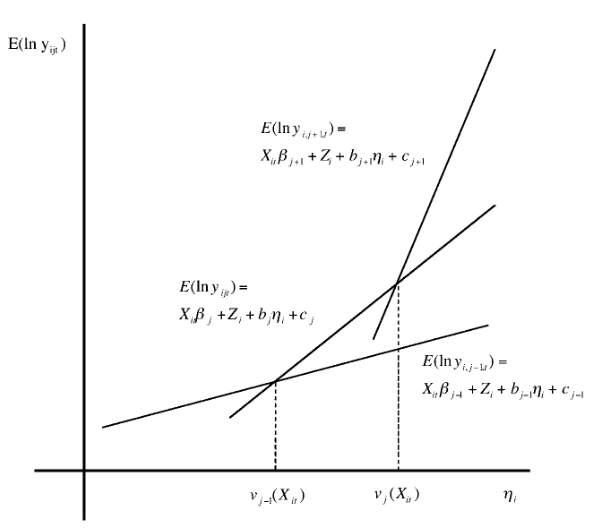
\includegraphics{gibbonsComparativeAdvantageLearning2005_fig1.png}}
        \label{gibbonsComparativeAdvantageLearning2005_fig1}
    \end{center}
\end{figure}

We again analyze first perfect and then imperfect information. In the perfect information case, firms in sector $j$ bid worker $i$'s wage up to the expected output in that sector:
\begin{equation}
    \label{9}
    \ln w_{i j t}=X_{i t} \beta_j+Z_i+b_j \eta_i+c_j+(1 / 2) b_j^2 \sigma_{\varepsilon}^2,
\end{equation}
analogous to (\ref{5}) but with the sector-specific returns $\b_j$ and $b_j$. \footnote{In this model, the sector-specific intercepts are now $c_j$ plus the term $\bp{1/2} b_j^2 \s_\ve^2$. This additional term accounts for the fact that when wages are paid in advance, differences in the variance of productivity across sectors (due to differences in the returns to skill $b_j$) lead to systematic differences in mean log wages because of the log normal transformation mentioned earlier. We view this as just one among several other possible sources of systematic wages differences across sectors. Other possible factors include compensating differentials, efficiency wages, and rents.} \highlightP{If the worker faces no mobility constraints, worker $i$ will choose to work in sector $j$ if $v_{j-1}\of{X_{it}} < \eta_i < v_{j}\of{X_{it}}$.} Thus, taking the model literally, sector mobility in the perfect information case is driven entirely by changes in $X_{it}\b_j$. One could envision exogenous shocks to sector demand that produce additional sector mobility in this model, but we will not formally model such shocks for the same reason that we did not model queues or rationing in Section II.A: our ultimate interest is in the model with comparative advantage and learning, which gives a coherent account of sectoral mobility without reference to queues, rationing, or sectoral shocks. Whatever the reason that worker $i$ is employed in sector $j$ in period $t$, in the perfect information case with comparative advantage, we assume that the worker's wage is given by (\ref{9}).

In the imperfect information case, we again assume that information in the labor market is symmetric but imperfect. As in the model of learning without comparative advantage, all participants in the labor market share the prior belief that $\eta_i$ is normal with mean $m$ and precision $h$, conditional on their initial information $Z_i$ and $X_{it}$. Inferences from the productivity observations, $y_{ijt}$, are greatly simplified because the information content of an output observation is constant across sectors; that is, (\ref{2}) involves $b_j\bp{\eta_i + \ve_{ijt}}$ rather than $b_j \eta_i + \ve_{ijt}$. This functional form is what allows us to define the normalized productivity observation for worker $i$ in period $t$, $s_{it}$ from (\ref{3}), to be a noisy signal about the worker's ability that is independent of the worker's sector during period $t$. Relaxing this assumption about the functional form of (\ref{2}) would complicate the analysis because workers' sector choices would then depend on the benefit from faster learning, as well as on the benefit from increased expected output given current beliefs. Relaxing the assumption that all labor market participants observe $Z_i$ (so that there could be learning about both $Z_i$ and $\eta_i$) would cause similar complications. \highlightP{Under our assumptions, the posterior distribution of $\eta_i$ given the history sit is normal with mean $m_{it}$ given by (\ref{4}) and precision $h_t = h + t h_{\ve}$, regardless of the worker's history of sector affiliations.}

In this fourth model, with learning and comparative advantage, we finally have an internally consistent account for sector affiliation, wages, sector mobility, and wage changes, as follows. In each period, firms in sector $j$ bid a worker's wage up to the worker's expected output in that sector, conditional on the publicly observable information about the worker available at that date:
\begin{equation}
    \label{10}
    \ln w_{i j t}=X_{i t} \beta_j+Z_i+b_j m_{i, t-1}+c_j+(1 / 2) b_j^2 \sigma_t^2
\end{equation}
which is analogous to (\ref{6}) but with sector-specific returns $\b_j$ and $b_j$. The model also includes sector-specific effects since the posterior variance $\s_t^2$, which declines with time (labor market experience), is interacted with $b_j^2$. The worker chooses to work in the sector offering the highest current wage. Thus, worker $i$ chooses sector $j$ in period $t+1$ if $v_{j-1}\left(X_{i, t+1}\right)<m_{i t}<v_j\left(X_{i, t+1}\right)$. In all of our models, including this richest one, if the parameters $\bc{\b_j, b_j, c_j; j = 1, \ldots, J}$ and the measured characteristics $X_{it}$ take on certain values, then one or more sectors may lie below the upper envelope in Figure \ref{gibbonsComparativeAdvantageLearning2005_fig1} for all values of the unmeasured characteristics, in which case no workers with such measured characteristics should be employed in such sectors.

\subsection{Estimation with Comparative Advantage}

We are now ready to develop a nonlinear instrumental variables procedure to estimate the parameters $\bc{\b_j, b_j, c_j; j = 1, \ldots, J}$ in (\ref{9}) and (\ref{10}). This procedure does not rely on normality. To discuss the estimation of the model, define the sector indicators $D_{ijt}$, where $D_{ijt}$ equals one if person $i$ is employed in sector $j$ at time $t$ and zero otherwise. 

The wage equation (\ref{10}) for each sector $j$ can then be written as a single equation where measurement error is assumed to be independent of sector affiliation:
\begin{equation}
    \label{11}
    \begin{aligned}
    \ln w_{i t}= & \sum_j D_{i j t} c_j+\sum_j D_{i j t} X_{i t} \beta_j+Z_i \\
    & +\sum_j D_{i j t} b_j m_{i, t-1}+(1 / 2) \sum_j D_{i j t} b_j^2 \sigma_t^2+\mu_{i t} .
    \end{aligned}
\end{equation}

Estimates of the sector slopes and intercepts $\bc{\b_j, c_j; j = 1, \ldots, J}$ obtained by estimating equation (\ref{11}) with OLS are inconsistent. The problem is that expected ability influences sector affiliation, so $m_{i, t-1}$ is correlated with the set of sector dummies $\bc{D_{ijt}, j = 1, \ldots, J}$. If the worker's ability were fixed, known, and equally valued in all sectors, then a first-differenced regression would eliminate this ability bias. But the endogeneity problem in equation (\ref{11}) is different from the usual fixed-effect case for two reasons. First, $m_{i,t-1}$ is a martingale rather than a fixed effect. This martingale property does not depend on the normality assumptions in our theoretical model; all Bayesian beliefs are martingales. In the absence of comparative advantage, we could handle this martingale problem as described in Section 2.2. But, second, comparative advantage causes $m_{i,t}$ to be interacted with the set of sector dummies $\bc{D_{ijt}, j = 1, \ldots, J}$.

\highlightR{SKIPPED FOR NOW!}


\section{Conclusion}

Broadly speaking, the results suggest that the measured occupational wage differentials in a cross-section regression are largely due to unmeasured and unobserved worker skills. We fine evidence that the sorting of skills into ``high-wage'' occupations is explained by high returns to skills in these occupations. Although comparative advantage appears to play a fundamental role in occupational wage differences, the role of learning is more limited. One possible explanation for this finding is that though learning may be quite important in the first few years in the labor market, it may not be as important later on.






\bibliography{\CiteReference}





\end{document}
